\documentclass[12pt]{article}
\usepackage{graphicx}
\usepackage{caption}
\usepackage{float}
\usepackage[a4paper,margin=1in,footskip=0.25in]{geometry}
\usepackage{pdfpages}
\usepackage{setspace}
\doublespace
% \usepackage[english]{babel}
% \usepackage[style=ieee,backend=biber]{biblatex}
% \addbibresource{lab.bib}
\usepackage{hyperref}
\hypersetup{
    colorlinks,
    citecolor=black,
    filecolor=black,
    linkcolor=black,
    urlcolor=black
}

\begin{document}

\title{Polyopticon SDS}
\author{Jon Bakies \and Mitchell Dunn} 

\maketitle
\newpage

\tableofcontents
\newpage

\section{Summary Of Proposal}
\paragraph{}
Polyopticon is a portable presentation tool that consists of a projector, camera, Raspberry Pi, and an infrared LED drawing tool.
The camera, pointed at the projected surface, will capture the user's pen strokes with image recogintion of the IR LED.
Originally the Raspberry Pi was intended to project and handle all of the image processing, but after testing it was determined that the Raspberry Pi could not handle such a demanding task.
Instead of performing the image recognition on the Raspberry Pi, the Pi will stream the video to the user's computer to be processed.

\section{Design}
\subsection{Image Recognition}
\subsubsection{Whiteboard}
\begin{figure}[ht!]
\centering
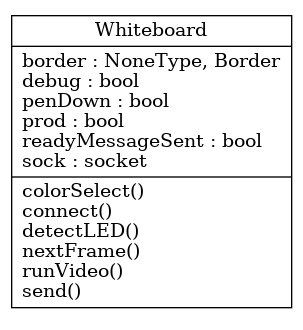
\includegraphics{whiteboard.png}
\end{figure}

\subsubsection{Border}
\begin{figure}[ht!]
\centering
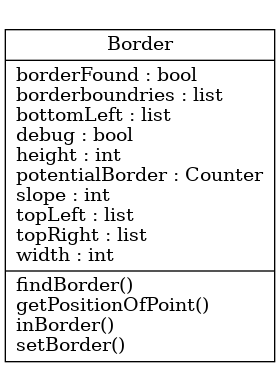
\includegraphics{border.png}
\end{figure}

% \newpage \section{References} \printbibliography[heading=none]
\end{document}
